\section{TPS-ZKPI Design}
\label{sec:design}

\subsection{Overview}

As shown in Figure~\ref{fig:tps-zkpi-workflow}, the TPS-ZKPI workflow binds a provider-committed hidden policy to requester-submitted authorization evidence through TPS-side proof generation and on-chain proof verification.
The provider registers only a policy commitment on-chain and sends policy-bound proving material to the TPS off-chain.
For each access request, the TPS constructs the private witness from the hidden policy material and requester evidence, generates a zero-knowledge proof of policy compliance, and submits a fixed-format proof statement for ACM verification.
The ACM records the authorization outcome in contract storage and emits it in the blockchain event log (as access-granted or access-denied events); the data access layer consumes this recorded decision to serve or refuse the request.

This design separates confidentiality-sensitive proof generation from public verification.
Policy material and requester evidence remain off-chain---policy material within the provider--TPS boundary, requester evidence between the requester and the TPS---while the blockchain verifies only a fixed-format proof statement against the provider's policy commitment, alongside session parameters validated by the ACM.
In a traditional requester-as-prover design, the requester generates the proof itself and must therefore receive the encoded policy and the commitment-opening randomness, so every requester learns the policy in normal operation.
In TPS-ZKPI, this material never leaves the provider--TPS boundary: the requester receives no policy material, and policy confidentiality can fail only if the TPS trust assumption itself is violated.

\begin{figure}[H]
	\centering
	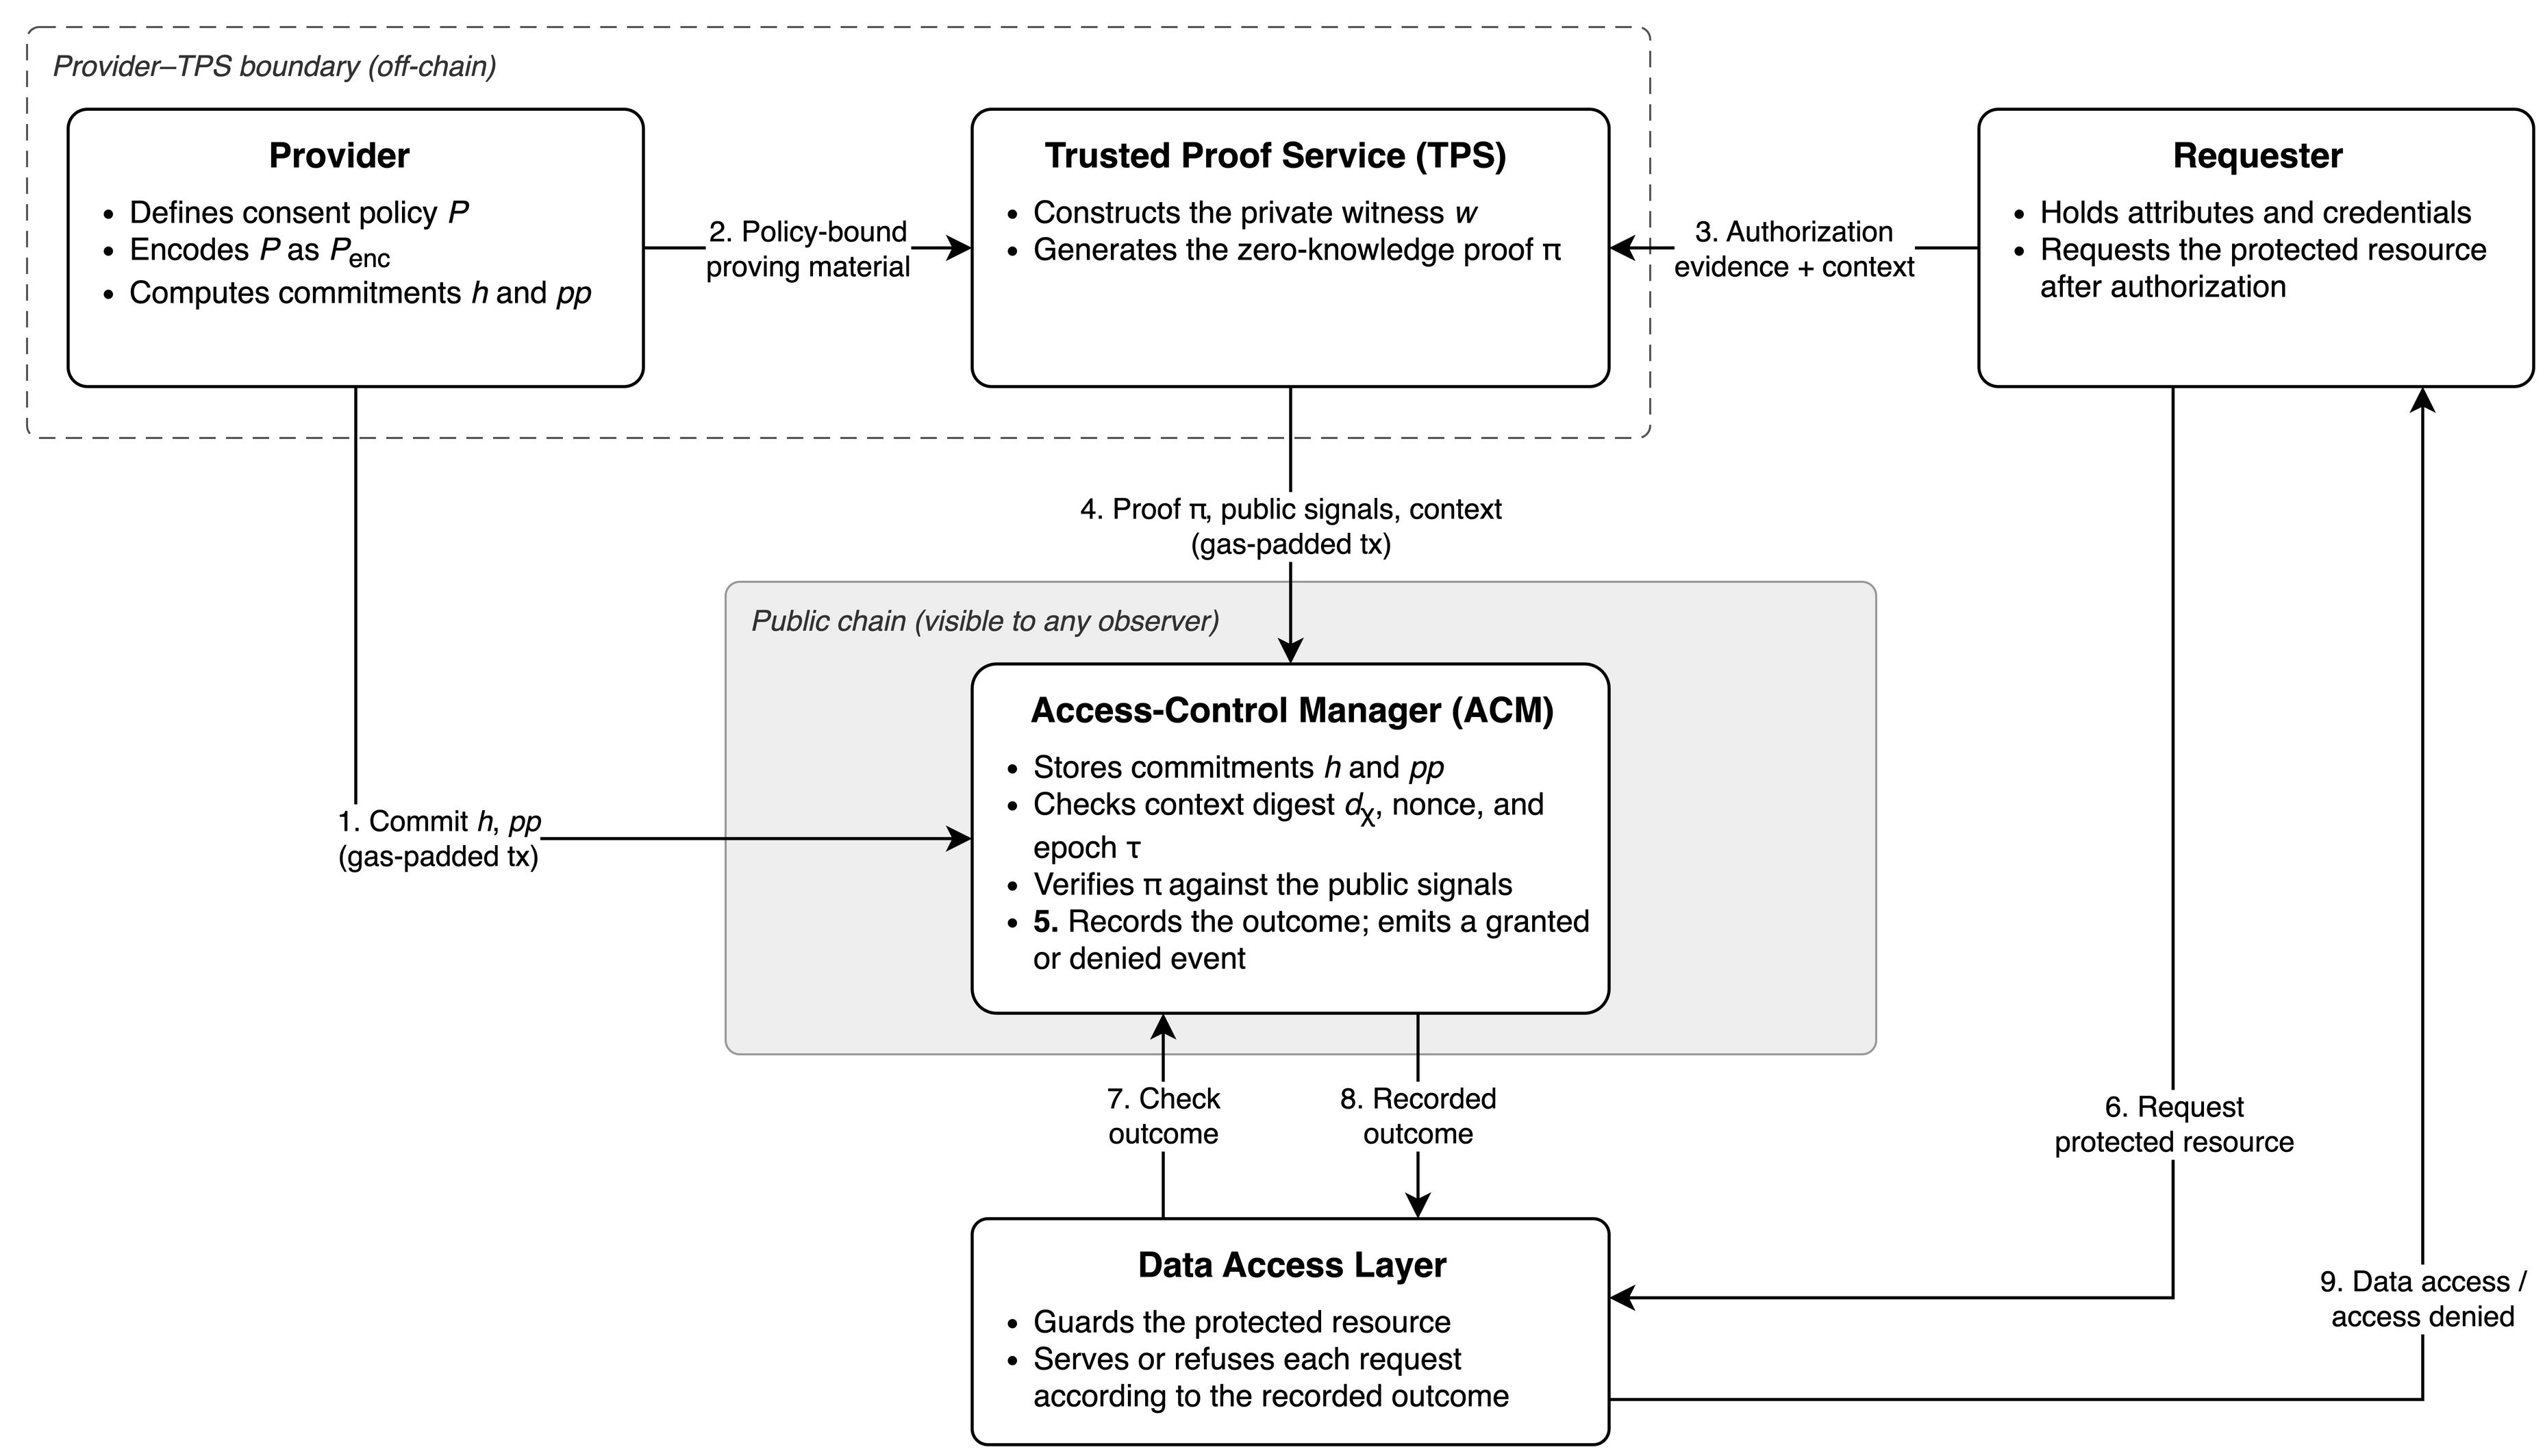
\includegraphics[width=0.9\textwidth]{PP-TPS.png}
	\caption{TPS-assisted policy-compliance workflow. The provider commits to the encoded policy on-chain and provisions proving material to the TPS (steps 1--2); the TPS constructs the witness from requester evidence and generates the proof (3--4); the ACM verifies the proof and records the outcome (5); the data access layer consults the recorded status to serve the requester (6--9).}
	\label{fig:tps-zkpi-workflow}
\end{figure}

\subsection{Policy Representation and Interpretation}

TPS-ZKPI represents heterogeneous Boolean-based consent policies in a fixed-length, circuit-friendly format.
This policy class is chosen for two reasons.
First, the targeted biomedical consent conditions---DUO-style data-use terms, disease-scope constraints, and institutional or ethics requirements---are categorical conditions combined with AND/OR/NOT, and conditions that are not natively Boolean, such as temporal validity or credential status, enter as externally attested predicate outcomes.
Second, a Boolean policy class admits a fixed-length encoding evaluated by a single reusable interpreter circuit, which keeps the verification interface policy-independent---a prerequisite for the privacy objectives evaluated later.
Let
\begin{equation}
	X = \{0,1\}^{N}, \qquad B = \{0,1\}^{M}
\end{equation}
denote the requester-attribute assignment space and the external-predicate assignment space, respectively.
The full assignment space is
\begin{equation}
	O = X \times B,
\end{equation}
where $a \in X$ encodes requester attributes and $b \in B$ encodes externally attested predicate outcomes, such as credential validity, ontology-linked checks, or obligation-related conditions.
Credential issuance, revocation, and attestation themselves remain external functions (Section~\ref{subsec:trust-model}): TPS-ZKPI consumes their outcomes as predicate bits and, where applicable, checks the associated auxiliary witnesses inside the proof relation.

Ontology-linked conditions are represented extensionally rather than through in-circuit ontology reasoning.
At encoding time, the provider expands an ontology concept into a whitelist of codes and commits the whitelist as a Merkle root among the policy's per-predicate parameters; in-circuit, the predicate check is a set-membership proof of the requested term against this root.
A disease-specific policy scoped to diabetes, for example, whitelists the ICD-10 diabetes subtree, whereas one scoped to type-1 diabetes whitelists only the type-1 codes.
Resolving subsumption at encoding time keeps ontology reasoning out of the circuit and preserves the policy-independent interface.

Consent policies are expressed as Boolean formulas over assignment bits:
\begin{equation}
	P ::= \mathit{atom} \mid (P \land P) \mid (P \lor P) \mid \neg P,\qquad
	\mathit{atom} ::= x_i \mid y_j .
\end{equation}
Here $x_i$ selects requester-attribute bit $a_i$ and $y_j$ selects external-predicate bit $b_j$.
For example, the consent condition ``the resource may be used for disease-specific research on diabetes, or for clinical care under approved clinical terms'' is expressed as $(x_1 \land y_1) \lor (x_2 \land y_2)$, where $x_1$ and $x_2$ flag the disease-specific-research and clinical-care purposes among the requester attributes, $y_1$ attests that the requested disease code lies in the committed diabetes whitelist, and $y_2$ attests that the requested clinical term lies in the approved clinical whitelist.
Each policy is compiled into a Reverse Polish Notation (RPN) program over operand tokens and Boolean operator tokens.
RPN linearizes arbitrarily nested formulas into a parenthesis-free token sequence that a stack machine evaluates in a single left-to-right pass with a fixed step count---a control structure that maps directly onto a fixed-size circuit and lets one interpreter serve all policies.
To support reusable verification, each program is padded to a fixed token length $L$:
\begin{equation}
	P_{\mathrm{enc}}= [t_{1},\ldots,t_{L}],
\end{equation}
together with an explicit program length $\ell \le L$ carried as a private witness.
The interpreter evaluates only the first $\ell$ tokens; padding positions beyond $\ell$ are inactive and leave the output unchanged.
The example policy above compiles to the token sequence $[x_1,\, y_1,\, \land,\, x_2,\, y_2,\, \land,\, \lor]$ with $\ell = 7$; the remaining $L-7$ positions are padding.
The implemented RC1 circuit uses $N=13$, $M=11$, and $L=\DEPTH=64$.
We denote the set of length-$L$ programs by $\mathsf{Prog}_{L}$.

The reusable policy interpreter is a zero-knowledge circuit
\begin{equation}
	C : \mathsf{Prog}_{L}\times \{0,\ldots,L\} \times O \rightarrow \{0,1\}.
\end{equation}
Given an encoded policy, its program length, and operand values, the interpreter evaluates the
RPN program using deterministic stack semantics and enforces well-formedness constraints inside the circuit.
The circuit outputs $1$ only if the requester evidence satisfies the encoded policy.
Well-formedness is enforced as hard constraints: for a program that violates the stack discipline, no satisfying witness exists and no proof can be generated.
An output of $0$ therefore indicates unsatisfied evidence for a well-formed program. The proved acceptance relation is the asserted case $C(P_{\mathrm{enc}},\ell,(a,b))=1$.

The fixed-length interpreter thus realizes the policy-independent interface motivated above, and supports policy evolution through different fixed-length policy programs.

\subsection{Commitment Binding and Proof Generation}

To bind each proof to a provider-defined hidden policy, the provider samples commitment randomness $r$ uniformly from the scalar field and computes
\begin{equation}
\begin{split}
	q &= \mathsf{H}_{\mathrm{pol}}(P_{\mathrm{enc}}),\\
	h &= \mathsf{Com}(P_{\mathrm{enc}},\ell; r)
	   = \mathsf{Poseidon}(q\parallel \ell\parallel r),
\end{split}
\end{equation}
where $q$ is the Poseidon-based digest of the fixed-length encoded policy, $\ell$ is the private program length, $r$ is the commitment randomness, and $h$ is the policy commitment stored on-chain.
The semantics of an encoded policy are determined by the pair $(P_{\mathrm{enc}},\ell)$, since $\ell$ identifies the active prefix of the padded token array.
Accordingly, the circuit supplies the same private value $\ell$ to both the commitment verifier and the policy interpreter.
Under the collision resistance of Poseidon, an accepting proof bound to $h$ cannot substitute a different program length and therefore cannot evaluate an alternative stack-consistent prefix of $P_{\mathrm{enc}}$.
Hiding is an explicit commitment assumption (Section~\ref{subsec:trust-model}) that relies on
high-entropy $r$ and the fixed-length encoding of $P_{\mathrm{enc}}$, which keeps the sponge input unambiguous.

For an access request, let
\begin{equation}
	\chi=(\mathit{id}_{\mathrm{req}},\mathit{id}_{\mathrm{res}},\nu),
	\qquad
	d_{\chi}=\mathsf{Poseidon}(\mathit{id}_{\mathrm{req}}\parallel
	\mathit{id}_{\mathrm{res}}\parallel\nu),
\end{equation}
where $\nu$ is a fresh session nonce.
The TPS constructs the private circuit witness
\begin{equation}
	w = (P_{\mathrm{enc}}, \ell, a, b, r, \omega, \chi),
\end{equation}
where $P_{\mathrm{enc}}$ is the encoded policy, $\ell$ is its program length, $a$ denotes requester attributes, $b$ denotes external predicate outcomes, $r$ is the commitment randomness, and $\omega$ denotes auxiliary witnesses for credential- or predicate-dependent checks.
The context tuple $\chi$ consists of private circuit inputs, while its digest $d_{\chi}$ is public.
The current public-signal vector is
\begin{equation}
	(1,h,\mathit{pp},d_{\chi},\tau),
\end{equation}
where $\mathit{pp}$ is a fixed-format commitment to the per-predicate parameters and $\tau$ is the request epoch used by the temporal checks.
Although the three components of $\chi$ are not separate Groth16 public inputs, the ACM receives them as transaction parameters in order to recompute $d_{\chi}$; they are therefore visible in transaction calldata.

For the compiled circuit, the Groth16~\cite{groth2016size} setup produces the common reference string as a proving key and a verification key, once for the shared circuit:
\begin{equation}
	(\mathit{pk}, \mathit{vk}) \leftarrow \mathsf{Setup}(C).
\end{equation}
The TPS generates a proof
\begin{equation}
	\pi \leftarrow \mathsf{Prove}\bigl(\mathit{pk}, w; (1,h,\mathit{pp},d_{\chi},\tau)\bigr).
\end{equation}
The proof certifies the conjunction that $C(P_{\mathrm{enc}},\ell,(a,b))=1$, $h=\mathsf{Com}(P_{\mathrm{enc}},\ell;r)$, $d_{\chi}=\mathsf{Poseidon}(\chi)$, and required external-predicate checks are internally consistent with respect to the supplied parameters and placeholder gadgets.
In the current implementation, the issuer-signature check among these gadgets is a hash-based placeholder (a Poseidon consistency check that provides no unforgeability), so attribute-origin binding is not an in-circuit guarantee; its scope and implications are treated in Sections~\ref{sec:problem} and~\ref{sec:discussion}.
Before verifying $\pi$, the ACM checks that the resource is governed by the stated policy, that $\tau$ is current, that the nonce has not been used for the same requester--resource context, and that the digest recomputed from the transaction parameters equals the public signal $d_{\chi}$.
Thus, within one ACM deployment, a proof generated for one requester identifier, resource, and nonce cannot be accepted under a different tuple.
The ACM then verifies $\pi$ against $\mathit{vk}$ and records the outcome of each request: a positive authorization outcome requires both a valid proof and an asserted output of $1$; otherwise the request is recorded as a denial.
The policy encoding, commitment randomness, requester attributes, credential witnesses, and auxiliary proof material are not posted on-chain.

\subsection{Transcript Normalization}

Zero-knowledge proofs hide private witness values, but surrounding
blockchain artifacts may still leak policy-dependent information. TPS-ZKPI therefore
normalizes the public transcript so that different policies induce fixed or tightly
bounded observable profiles. Table~\ref{tab:transcript-normalization}
summarizes the mechanisms.

\begin{table}[H]
	\centering
	\caption{Transcript-normalization mechanisms in TPS-ZKPI.}
	\label{tab:transcript-normalization} \footnotesize
	\begin{tabular}{p{0.24\linewidth}p{0.66\linewidth}}
		\hline
		\textbf{Artifact} & \textbf{Normalization mechanism}                                                   \\
		\hline
		Calldata          & Fixed verification interface and fixed-size proof/public-input encoding.           \\
		Logs              & Fixed event structure with constant topic and payload layout.                      \\
		Public parameters & Fixed-format handles instead of policy artifacts or credential witnesses.          \\
		Gas usage         & Policy-independent verifier logic and randomized gas padding toward fixed targets. \\
		\hline
	\end{tabular}
\end{table}

These mechanisms do not eliminate all public observability. Rather, they reduce policy-dependent variation in calldata, logs, public parameters, and gas-related behavior that could otherwise serve as a fingerprint for the metadata-only adversary defined in Section~\ref{sec:problem}.
TPS-ZKPI does not flatten all residual channels: timing between transactions, transaction ordering, mempool or broadcast patterns, and off-chain TPS communication remain outside the normalized public transcript.
